\documentclass[12pt]{article}

\usepackage{amsmath,amsfonts,amsthm,amssymb}
\usepackage{color}
\usepackage{graphicx}
\usepackage{wrapfig}
\usepackage{epsfig}
%\usepackage{subfigure}
\usepackage{times}
\usepackage{xspace}
\usepackage{url}
\usepackage{pdfpages}
\usepackage{array}
\usepackage{subfig}
\usepackage{multirow}
\usepackage{dblfloatfix} 

\setlength{\topmargin}{0.0in}     % top of paper to head (less one inch)
\setlength{\headheight}{0in}      % height of the head
\setlength{\headsep}{0in}         % head to the top of the body
\setlength{\textheight}{9.0in}    % height of the body
\setlength{\oddsidemargin}{-.25in} % left edge of paper to body (less one inch)
\setlength{\evensidemargin}{0mm}  % ditto, even pages
\setlength{\textwidth}{7.0in}     % width of body
\setlength{\topskip}{0in}         % top of body to bottom of first line of text
\setlength{\parindent}{1pc}       

\begin{document}
\thispagestyle{empty}
%%%%%%%%%%%%%%%%%%%%%%%%%%%%%%%%%%%%%%%%%%%%%%%%%%%%%%%%%%%%%%%%%%%%%%%%%%%%%%%%%%%%%%%%
% Project Summary
%%%%%%%%%%%%%%%%%%%%%%%%%%%%%%%%%%%%%%%%%%%%%%%%%%%%%%%%%%%%%%%%%%%%%%%%%%%%%%%%%%%%%%%%
\begin{center}
{\Large\bf Project Update \#2}
\vspace{3mm}
\\Caitlin Ross, Noah Wolfe
\\4/21/2016
\\*[3mm]
\end{center}

\section{Data Collection}
As we started creating the interface, we realized that we need to make changes to our data collection again.  We are still collecting simulation level data, however, now we're collecting the data directly from the Slim Fly model (we'll add in dragonfly data as time permits), instead of ROSS itself.  Because of this, we've decided to limit to just the number of forward and reverse events, since we can collect this easily from the model.  In the future, we can provide hooks into ROSS to collect this data as well as other metrics directly from ROSS.  So now we are collecting data on the specific events that are sent between LPs (logical processes, or in other words the simulation entities) in the simulation, recording the source and destination LPs, the timestamp, and the type of event.  

We're also writing scripts to do some post-processing on this data that will be uploaded into our visualization interface.  We'll have two files.  One that stores the values for a given metric (e.g., number of forward events) for each LP.  These are aggregated into bins based on the GVT (Global Virtual Time) computations done during the simulation.  This file will be used for two of the visualization components. The other file stores the number of events per each PE pair for each GVT.  This file will be used for creating the radial diagram.  



\section{Interface Changes}
We are making two changes to our proposed interface. One change we discussed in our progress report last week.  This is to add a parallel coordinates graph to the top of the interface.  This presents an overview of all simulations performed and will allow a user to select one run out of the collection to update the rest of the interface.   The other change we plan to make is based on an example we found on the D3 examples pages.  Figure \ref{ross-view} shows the original interface.  The change we are making is to the LP View in the top right.  As seen in the figure, we planned to create a grid showing the LPs that would be a heat map based on the values of whatever metric we're viewing.  Now we plan to do something like this: \url{https://github.com/marmelab/EventDrops}.  We would modify this so that each row is an LP belonging to the selected PE (processing element).  Simulated time would replace the actual time in the example.  Then you could zoom in and out on the simulated time and see where events fall over time.

\section{Current Progress}
Noah is working on the post-processing script described above, while Caitlin is working on the interface.  Figure \ref{current} shows the current progress on the interface.  So far the parallel coordinates described in the previous selection is complete.  Currently it is showing a few lines of a dataset I made up.  Now I am working on finishing the time selection component.  For some reason I am having an issue with the lines being shoved to the right of the actual graph.  The next steps are to finish the Radial View and the LP Selector.  The LP View will be the last component, time permitting.  

\begin{figure*}[t]
\centering
   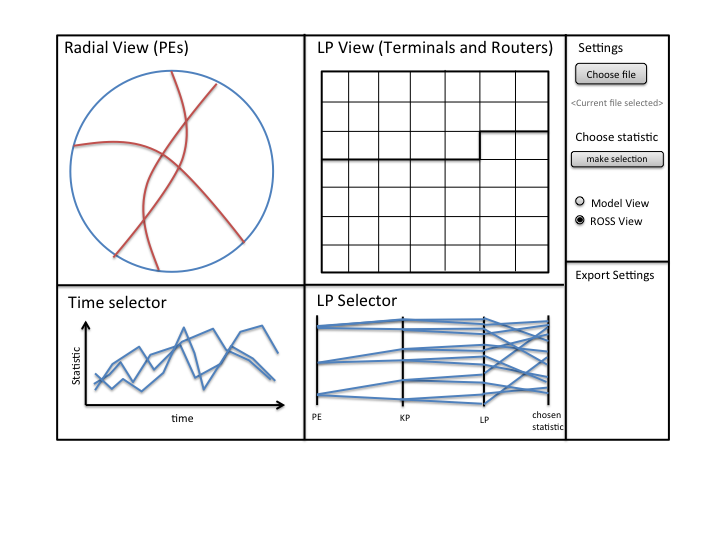
\includegraphics[width=6.5in, clip=true, trim=0 1in 0 0]{../../figures/gui-diagram/Slide2.png}
\caption{Originally Proposed Interface}
\label{ross-view}
\end{figure*}

\begin{figure*}[t]
\centering
   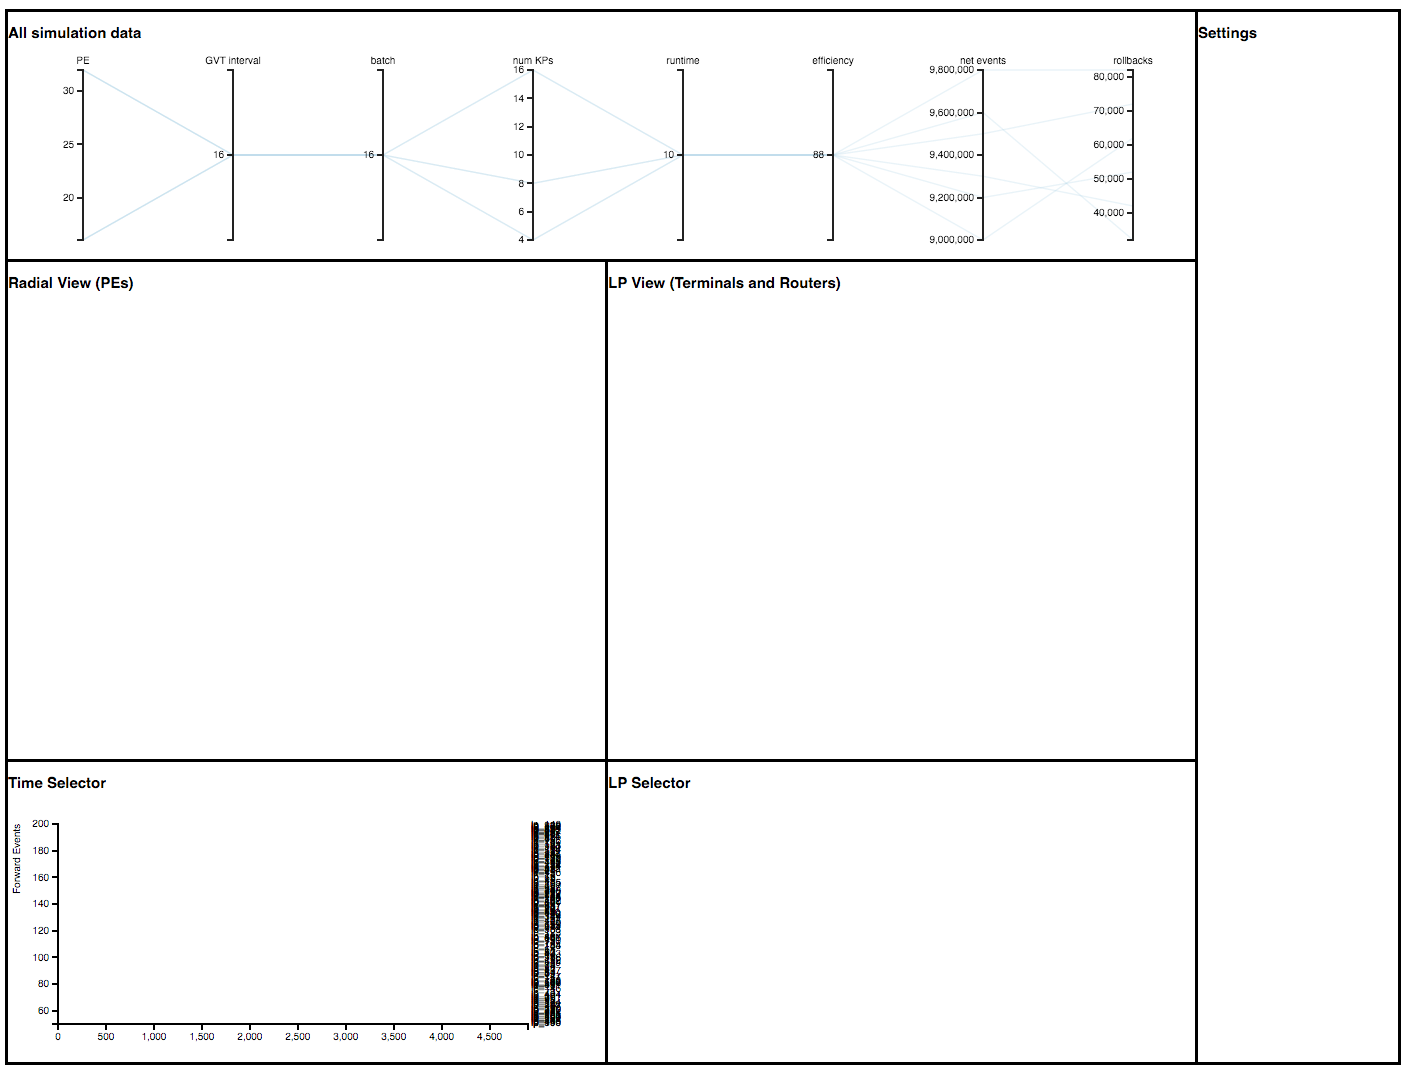
\includegraphics[width=6.5in]{current.png}
\caption{Current progress on interface}
\label{current}
\end{figure*}




%\end{document}  % This is where a 'short' article might terminate

%ACKNOWLEDGMENTS are optional
%\section{Acknowledgments}

%
% The following two commands are all you need in the
% initial runs of your .tex file to
% produce the bibliography for the citations in your paper.

% You must have a proper ".bib" file
%  and remember to run:
% latex bibtex latex latex
% to resolve all references
%
% ACM needs 'a single self-contained file'!
%
%APPENDICES are optional
%\balancecolumns


%\balancecolumns % GM June 2007
% That's all folks!
\end{document}
